\chapter{Pastas Time Series Modeling}
\label{appendix: A}

%\emph{Adding source code to your report/thesis is supported with the package {\normalfont\texttt{listings}}. An example can be found below. Files can be added using {\normalfont\texttt{\textbackslash lstinputlisting[language=<language>]\{<filename>\}}}.}

%\emph{The Pastas model describes how a basic time series model can be developed in order to simulate groundwater levels, either in the future or past. The hydrologic parameter 'recharge' is used as explanatory time series variable. Meaning that the variable is used to forecast the data instead of using historical data. Recharge is calculated according to the following formula: \\

%\[Recharge = Precipitation - Evaporation\]


\section{Results of Pastas time series modeling}
For stress model 1, the depicted figures explain a model summary based on the parameter \textit{recharge rate} for the case study areas Rozenburg and Heijplaat. The figure consists of 4 subplots and a summarizing table \cite{collenteur-2019}. The first plot visualizes the observed and simulated groundwater level data [m NAP] with a coefficient of determination [$R^2$] that compares the simulated data with the observed data. The second plot visualizes the residual and noise series of the model. The residuals can indicate if a certain stress is missing from the model, in a situation where a clear trend of the residuals is visible. The residuals are auto-correlated with extended periods, where the modeled heads are higher or lower than the observed heads, while the noise shows little auto-correlation. The third plot, below, plots the estimated recharge over the project period [m/day]. The fourth plot, on the bottom right side of the figure, shows the estimated step response that explains the increase in recharge rate to a final level of recharge rate [mm/day]. The table provides results of the fit report that is returned by the solve method and shows information on the model settings, the fit statistics, and the estimated parameters. The solve function has a number of default options that can be specified with keyword arguments. The fit report encompasses an overview of the fitting procedure, the optimal values obtained by the fitting routine, and basic statistics. \\
\noindent
\\
The model encloses five parameters: 1) \(A\); 2) \(n\); 3) \(a\); 4) \(d\); 5) \(\alpha\). The first three parameters are used as a \textit{Gamma} function as the response function for the recharge, parameter \textit{d} which indicates the constant base level, and parameter \(\alpha\) of the noise model that indicates if there is a significant difference between the auto-correlation in the noise. Overall, the model simulation shows a good fit with the observed groundwater levels in the calibration period if the model is supported by a low RMSE [cm] and a high Pearson $R^2$ value. \\
\noindent
\\
For stress model 1, the recharge rate was estimated as \(P\) minus \($E_a$\) \cite{collenteur-2019}. To improve the model, \($E_a$\) as a factor is estimated, times \($E_{\text{pot}}$\). Stress model 2 encompasses the precipitation and evaporation series with an additional parameter for the evaporation factor \(f\). Stress model 2 gives an improved representation and fit of the model \cite{collenteur-2019}. Meaning that the RMSE is lowered with a higher explained variance \($R^2$\). However, according to the Akaike Information Criterion, incorporating the evaporation factor \(f\) into the model does not significantly enhance the performance of the model. The depicted figures for stress model 2 are visualized from figure \labelcref{SM2: start} on.

\newpage
\subsection{Stress Model 1: Rozenburg}\\

\begin{figure}[htbp]
    \centering
    % First figure
    \begin{minipage}{0.32\textwidth}
        \centering
        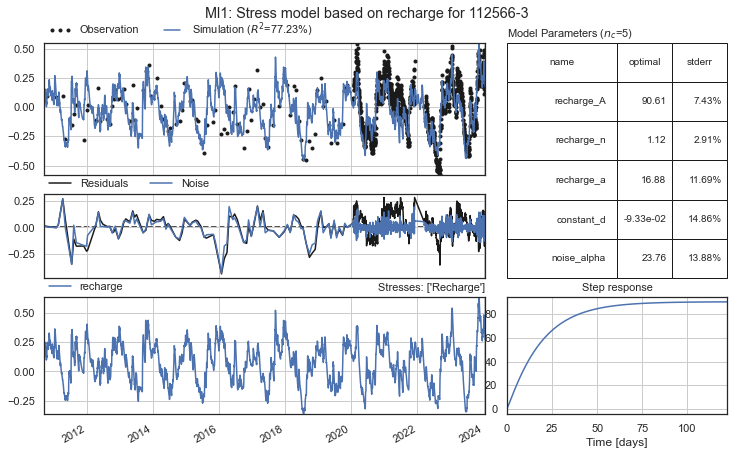
\includegraphics[width=\linewidth]{frontmatter/Rozenburg-fig/1.png}
        \caption{Monitoring well: 112566-3.}
        \label{fig:112565-3}
    \end{minipage}
    \hfill
    % Second figure
    \begin{minipage}{0.32\textwidth}
        \centering
        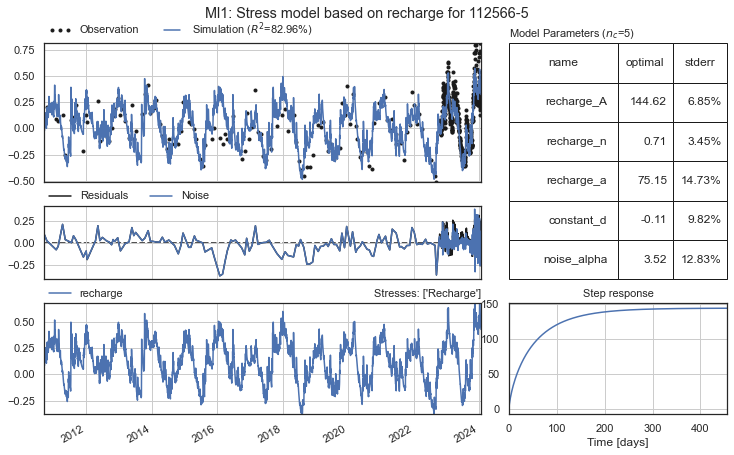
\includegraphics[width=\linewidth]{frontmatter/Rozenburg-fig/2.png}
        \caption{Monitoring well: 112566-5.}
        \label{fig:112565-3}
    \end{minipage}
    \hfill
    % Third figure
    \begin{minipage}{0.32\textwidth}
        \centering
        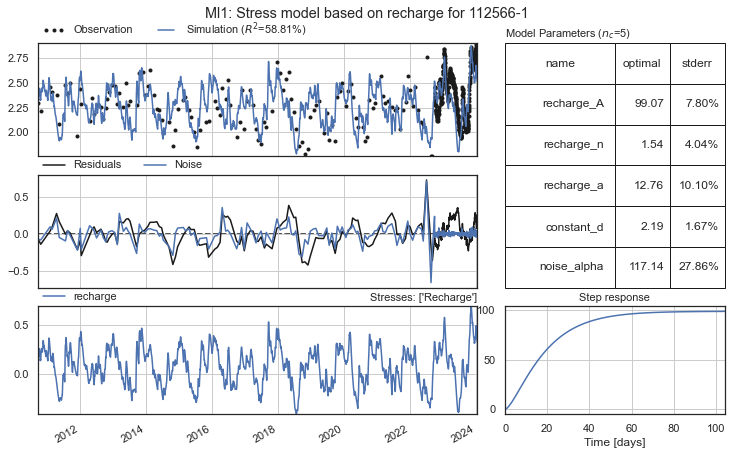
\includegraphics[width=\linewidth]{frontmatter/Rozenburg-fig/3.png}
        \caption{Monitoring well: 112566-1.}
        \label{fig:112565-3}
    \end{minipage}
\end{figure}

\begin{figure}[htbp]
    \centering
    % First figure
    \begin{minipage}{0.32\textwidth}
        \centering
        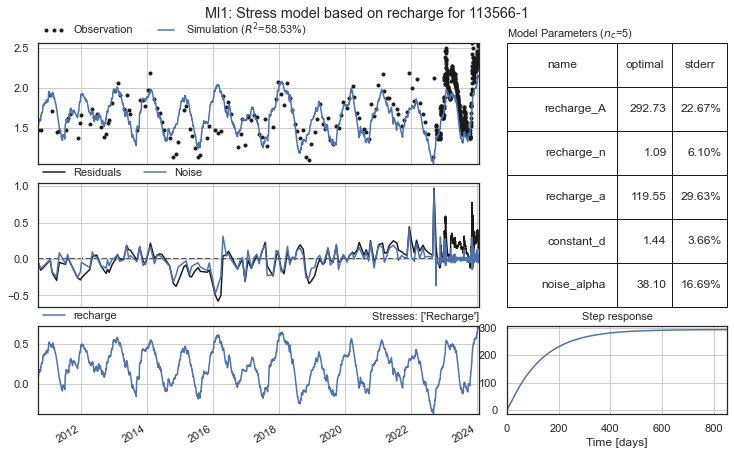
\includegraphics[width=\linewidth]{frontmatter/Rozenburg-fig/4.png}
        \caption{Monitoring well: 113566-1.}
        \label{fig:112565-3}
    \end{minipage}
    \hfill
    % Second figure
    \begin{minipage}{0.32\textwidth}
        \centering
        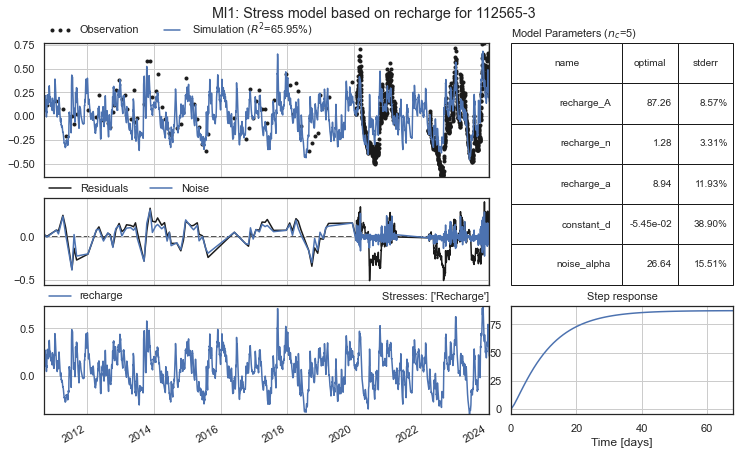
\includegraphics[width=\linewidth]{frontmatter/Rozenburg-fig/5.png}
        \caption{Monitoring well: 112565-3.}
        \label{fig:112565-3}
    \end{minipage}
    \hfill
    % Third figure
    \begin{minipage}{0.32\textwidth}
        \centering
        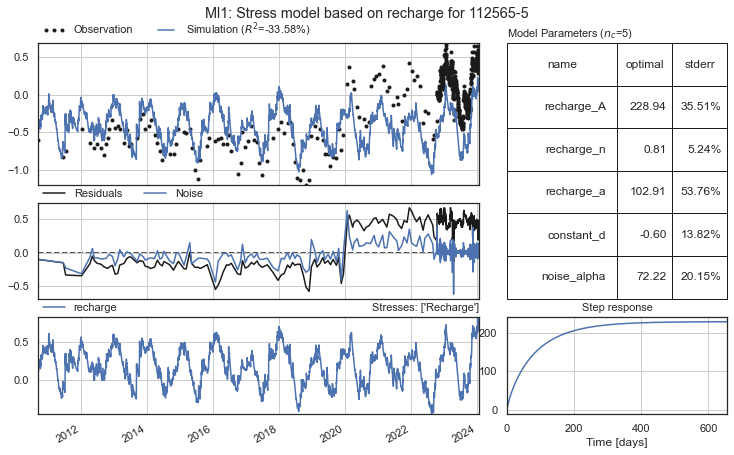
\includegraphics[width=\linewidth]{frontmatter/Rozenburg-fig/6.png}
        \caption{Monitoring well: 112565-5.}
        \label{fig:112565-3}
    \end{minipage}
\end{figure}

\begin{figure}[htbp]
    \centering
    % First figure
    \begin{minipage}{0.32\textwidth}
        \centering
        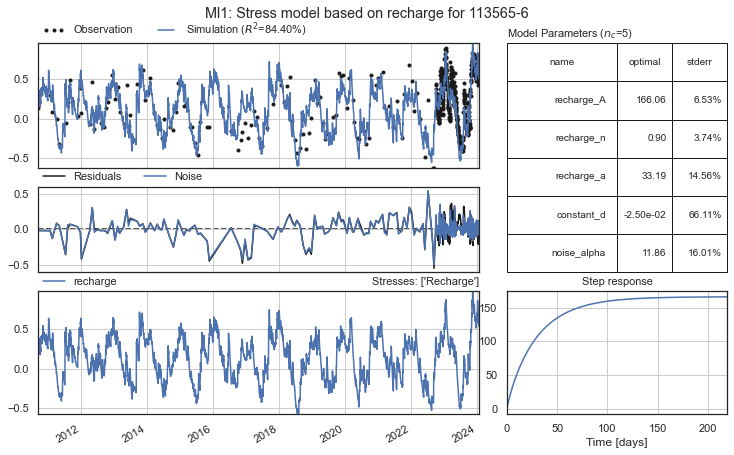
\includegraphics[width=\linewidth]{frontmatter/Rozenburg-fig/7.png}
        \caption{Monitoring well: 113565-6.}
        \label{fig:112565-3}
    \end{minipage}
    \hfill
    % Second figure
    \begin{minipage}{0.32\textwidth}
        \centering
        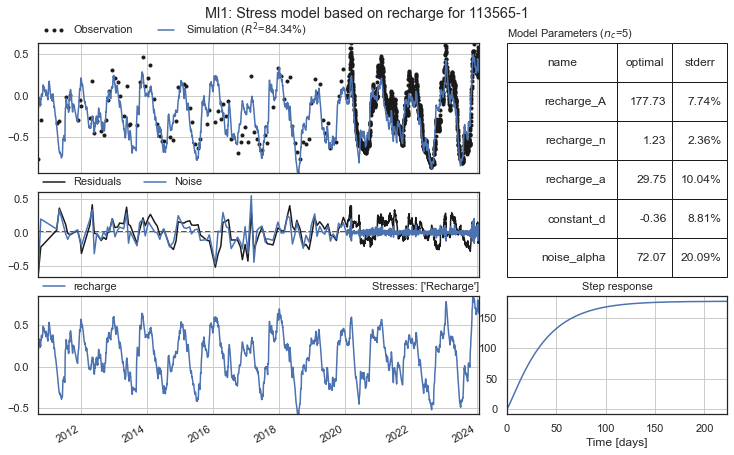
\includegraphics[width=\linewidth]{frontmatter/Rozenburg-fig/8.png}
        \caption{Monitoring well: 113565-1.}
        \label{fig:112565-3}
    \end{minipage}
    \hfill
    % Third figure
    \begin{minipage}{0.32\textwidth}
        \centering
        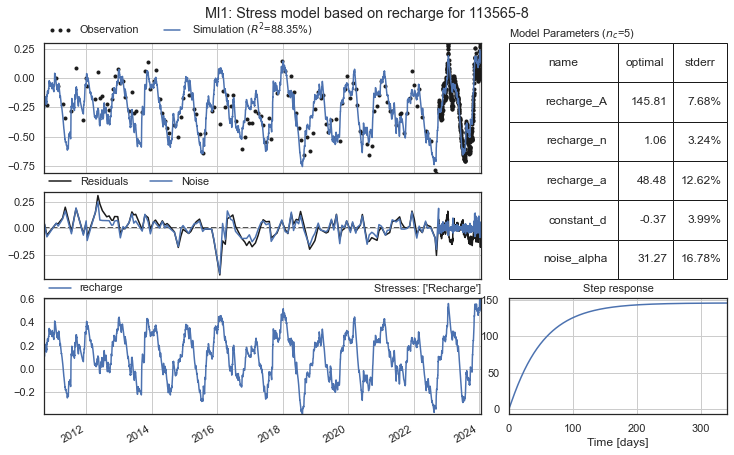
\includegraphics[width=\linewidth]{frontmatter/Rozenburg-fig/9.png}
        \caption{Monitoring well: 112565-8.}
        \label{fig:112565-3}
    \end{minipage}
\end{figure}
\begin{figure}[htbp]
    \centering
    % First figure
    \begin{minipage}{0.32\textwidth}
        \centering
        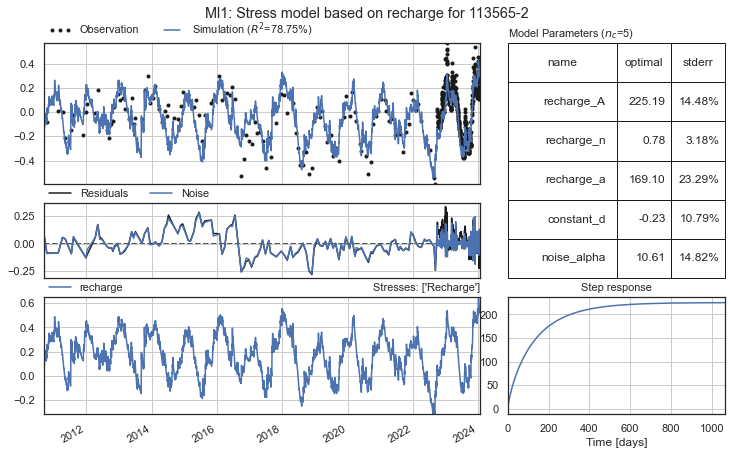
\includegraphics[width=\linewidth]{frontmatter/Rozenburg-fig/10.png}
        \caption{Monitoring well: 113565-2.}
        \label{fig:112565-3}
    \end{minipage}
    \hfill
    % Second figure
    \begin{minipage}{0.32\textwidth}
        \centering
        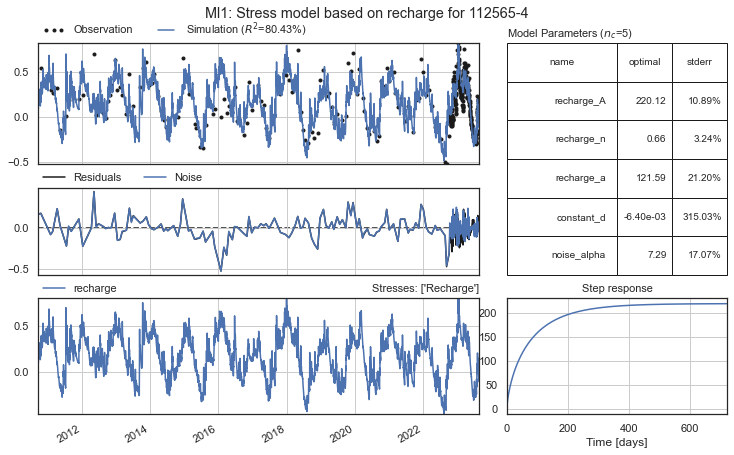
\includegraphics[width=\linewidth]{frontmatter/Rozenburg-fig/11.png}
        \caption{Monitoring well: 112565-4.}
        \label{fig:112565-3}
    \end{minipage}
    \hfill
    % Third figure
    \begin{minipage}{0.32\textwidth}
        \centering
        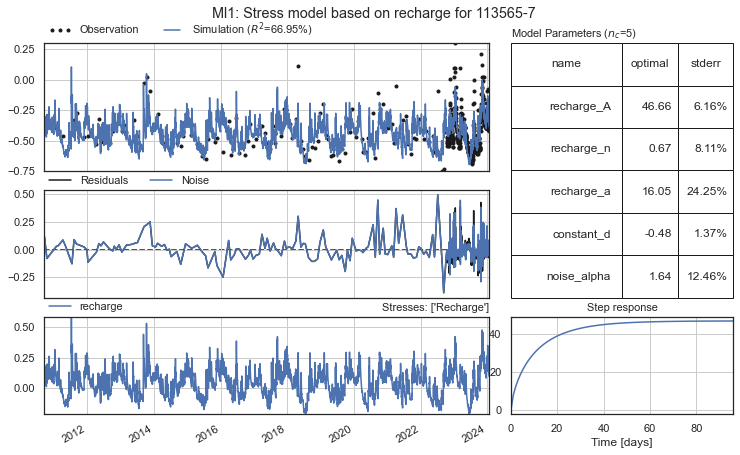
\includegraphics[width=\linewidth]{frontmatter/Rozenburg-fig/12.png}
        \caption{Monitoring well: 113565-7.}
        \label{fig:112565-3}
    \end{minipage}
\end{figure}

\begin{figure}[htbp]
    \centering
    % First figure
    \begin{minipage}{0.32\textwidth}
        \centering
        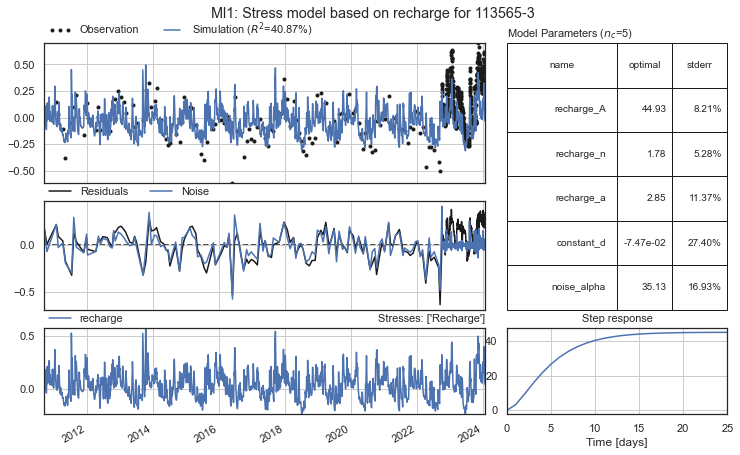
\includegraphics[width=\linewidth]{frontmatter/Rozenburg-fig/13.png}
        \caption{Monitoring well: 113565-3.}
        \label{fig:112565-3}
    \end{minipage}
    \hfill
    % Second figure
    \begin{minipage}{0.32\textwidth}
        \centering
        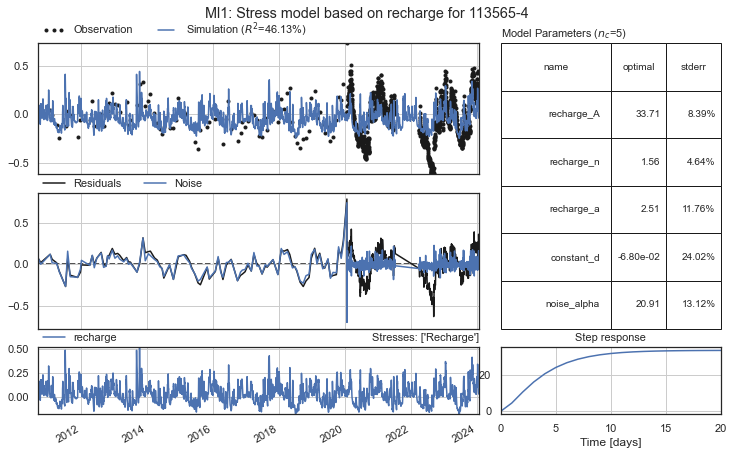
\includegraphics[width=\linewidth]{frontmatter/Rozenburg-fig/14.png}
        \caption{Monitoring well: 113565-4.}
        \label{fig:112565-3}
    \end{minipage}
    \hfill
    % Third figure
    \begin{minipage}{0.32\textwidth}
        \centering
        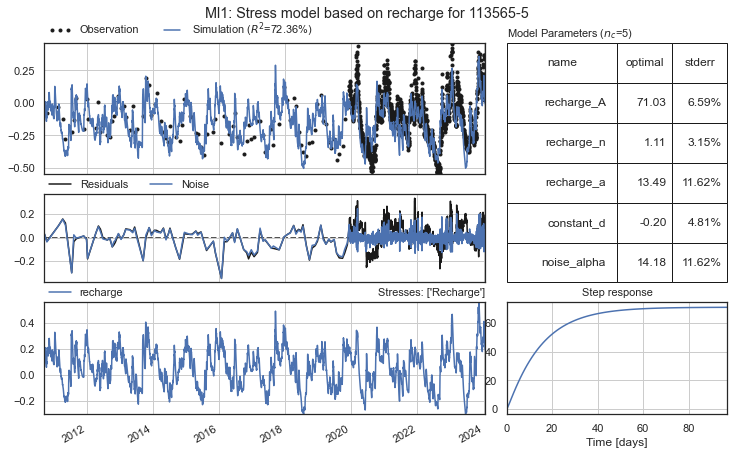
\includegraphics[width=\linewidth]{frontmatter/Rozenburg-fig/15.png}
        \caption{Monitoring well: 113565-5.}
        \label{fig:112565-3}
    \end{minipage}
\end{figure}
\begin{figure}[htbp]
    \centering
    % First figure
    \begin{minipage}{0.32\textwidth}
        \centering
        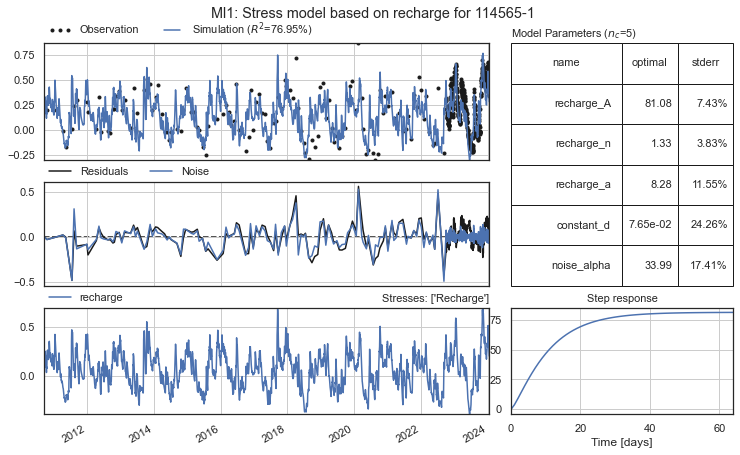
\includegraphics[width=\linewidth]{frontmatter/Rozenburg-fig/16.png}
        \caption{Monitoring well: 114565-1.}
        \label{fig:112565-3}
    \end{minipage}
    \hfill
    % Second figure
    \begin{minipage}{0.32\textwidth}
        \centering
        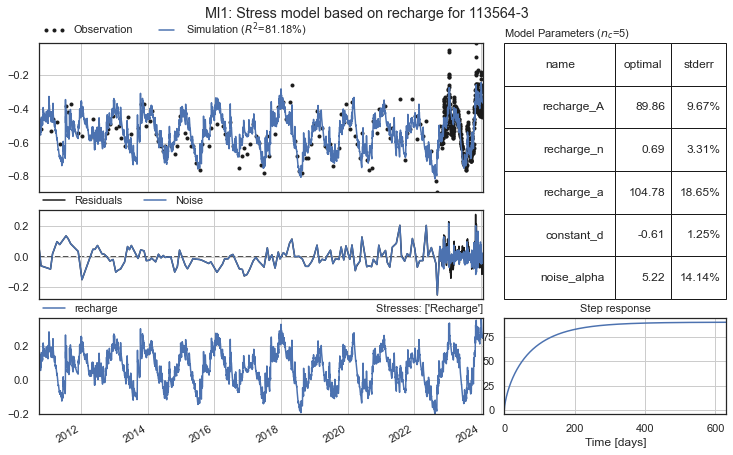
\includegraphics[width=\linewidth]{frontmatter/Rozenburg-fig/17.png}
        \caption{Monitoring well: 113564-3.}
        \label{fig:112565-3}
    \end{minipage}
    \hfill
    % Third figure
    \begin{minipage}{0.32\textwidth}
        \centering
        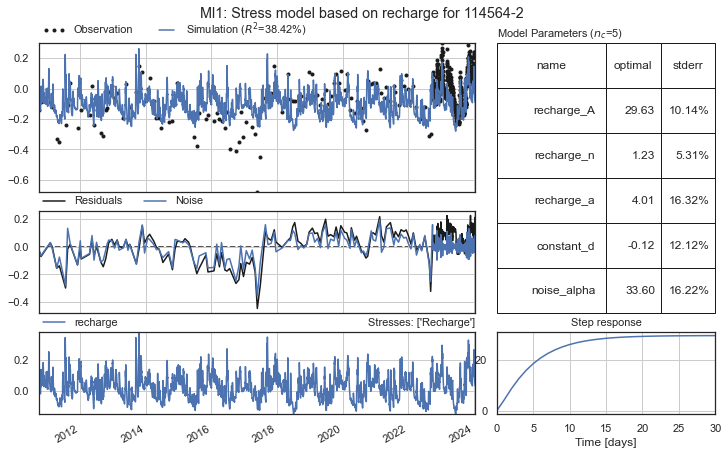
\includegraphics[width=\linewidth]{frontmatter/Rozenburg-fig/18.png}
        \caption{Monitoring well: 114564-2.}
        \label{fig:112565-3}
    \end{minipage}
\end{figure}
\begin{figure}[htbp]
    \centering
    % First figure
    \begin{minipage}{0.32\textwidth}
        \centering
        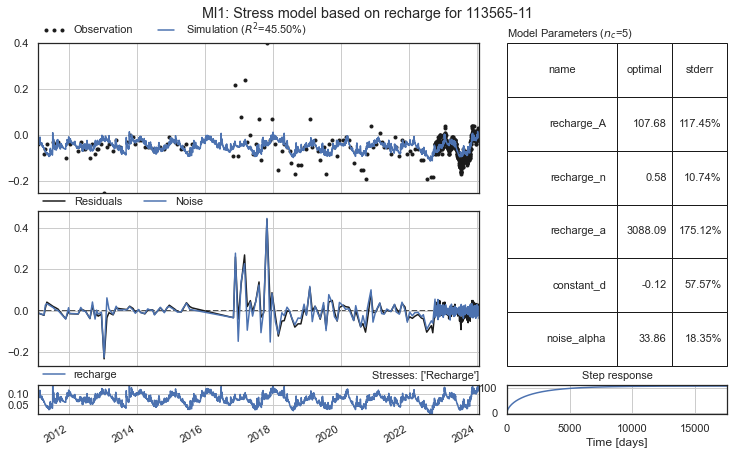
\includegraphics[width=\linewidth]{frontmatter/Rozenburg-fig/19.png}
        \caption{Monitoring well: 113565-11.}
        \label{fig:112565-3}
    \end{minipage}
    \hfill
    % Second figure
    \begin{minipage}{0.32\textwidth}
        \centering
        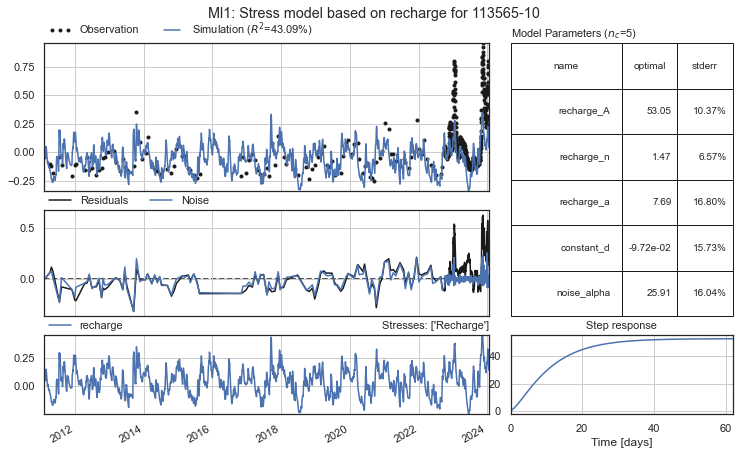
\includegraphics[width=\linewidth]{frontmatter/Rozenburg-fig/20.png}
        \caption{Monitoring well: 113565-10.}
        \label{fig:112565-3}
    \end{minipage}
    \hfill
    % Third figure
    \begin{minipage}{0.32\textwidth}
        \centering
        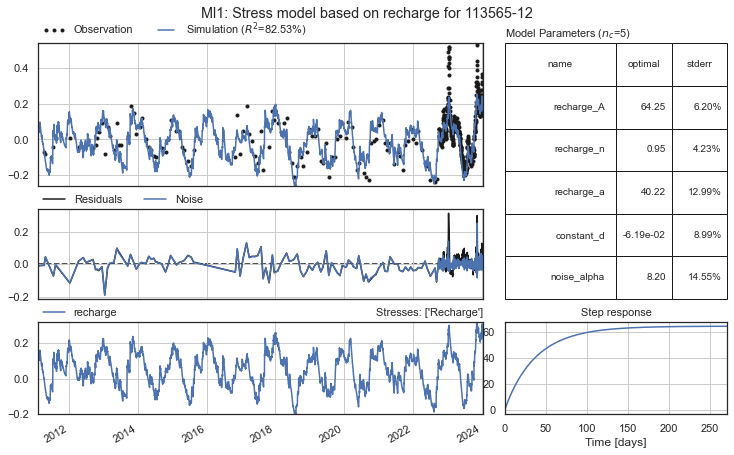
\includegraphics[width=\linewidth]{frontmatter/Rozenburg-fig/21.png}
        \caption{Monitoring well: 113565-12.}
        \label{fig:112565-3}
    \end{minipage}
\end{figure}
\begin{figure}[htbp]
    \centering
    % First figure
    \begin{minipage}{0.32\textwidth}
        \centering
        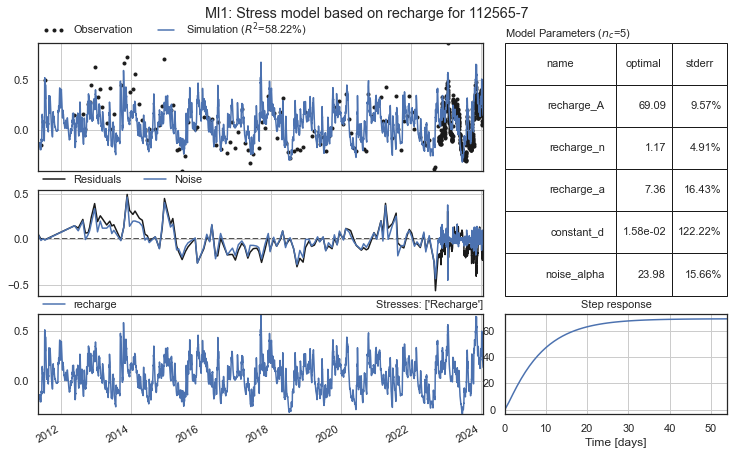
\includegraphics[width=\linewidth]{frontmatter/Rozenburg-fig/22.png}
        \caption{Monitoring well: 112565-7.}
        \label{fig:112565-3}
    \end{minipage}
    \hfill
    % Second figure
    \begin{minipage}{0.32\textwidth}
        \centering
        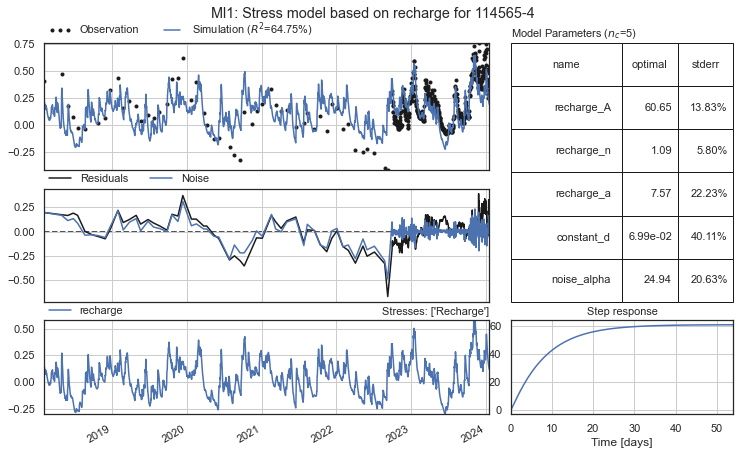
\includegraphics[width=\linewidth]{frontmatter/Rozenburg-fig/23.png}
        \caption{Monitoring well: 114565-4.}
        \label{fig:112565-3}
    \end{minipage}
    \hfill
    % Third figure
    \begin{minipage}{0.32\textwidth}
        \centering
        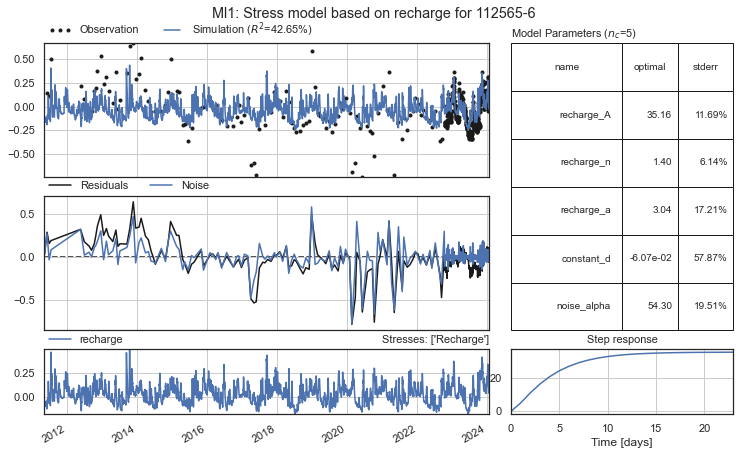
\includegraphics[width=\linewidth]{frontmatter/Rozenburg-fig/24.png}
        \caption{Monitoring well: 112565-6.}
        \label{fig:112565-3}
    \end{minipage}
\end{figure}
\begin{figure}[htbp]
    \centering
    % First figure
    \begin{minipage}{0.32\textwidth}
        \centering
        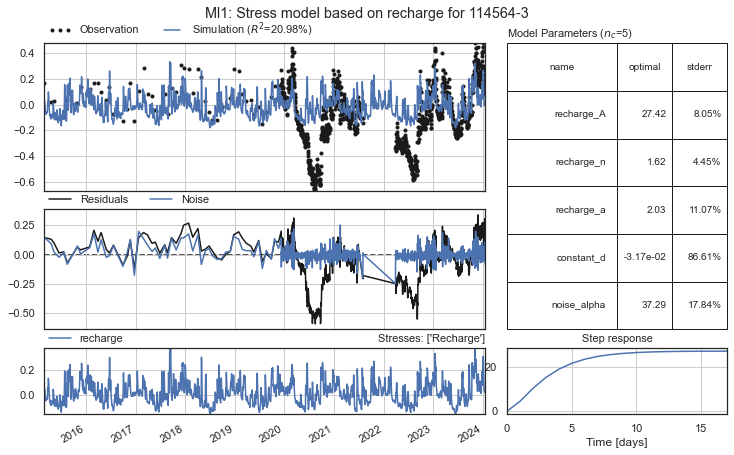
\includegraphics[width=\linewidth]{frontmatter/Rozenburg-fig/25.png}
        \caption{Monitoring well: 1145654-3.}
        \label{fig:112565-3}
    \end{minipage}
    \hfill
    % Second figure
    \begin{minipage}{0.32\textwidth}
        \centering
        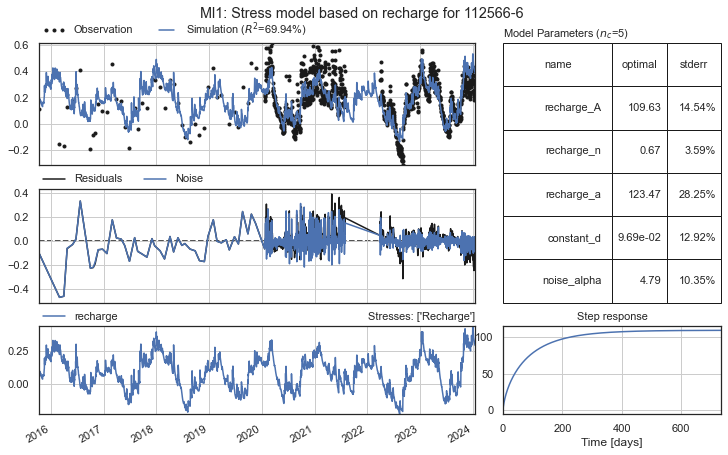
\includegraphics[width=\linewidth]{frontmatter/Rozenburg-fig/26.png}
        \caption{Monitoring well: 112566-6.}
        \label{fig:112565-3}
    \end{minipage}
    \hfill
    % Third figure
    \begin{minipage}{0.32\textwidth}
        \centering
        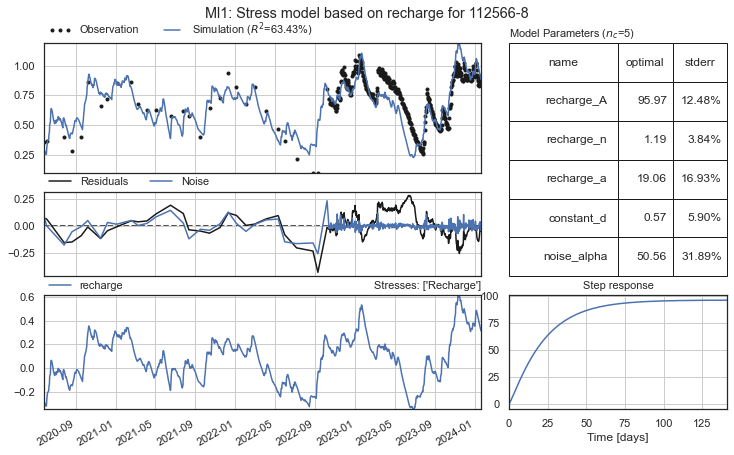
\includegraphics[width=\linewidth]{frontmatter/Rozenburg-fig/27.png}
        \caption{Monitoring well: 112566-8.}
        \label{fig:112565-3}
    \end{minipage}
\end{figure}

\begin{figure}[htbp]
    \centering
    % First figure
    \begin{minipage}{0.32\textwidth}
        \centering
        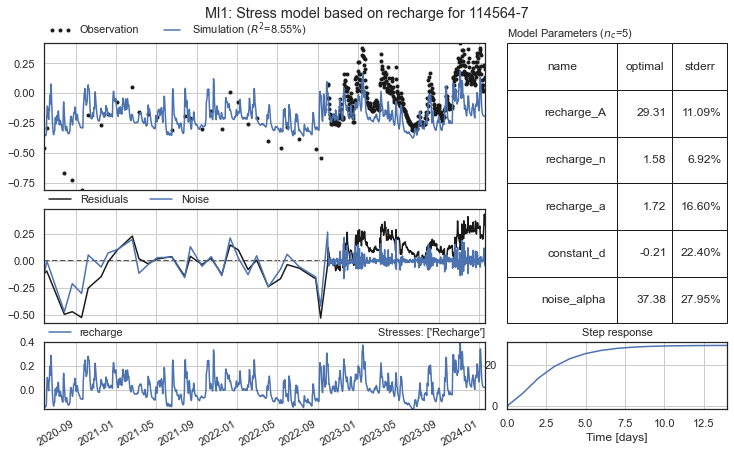
\includegraphics[width=\linewidth]{frontmatter/Rozenburg-fig/28.png}
        \caption{Monitoring well: 114564-7.}
        \label{fig:112565-3}
    \end{minipage}
    \hfill
    % Second figure
    \begin{minipage}{0.32\textwidth}
        \centering
        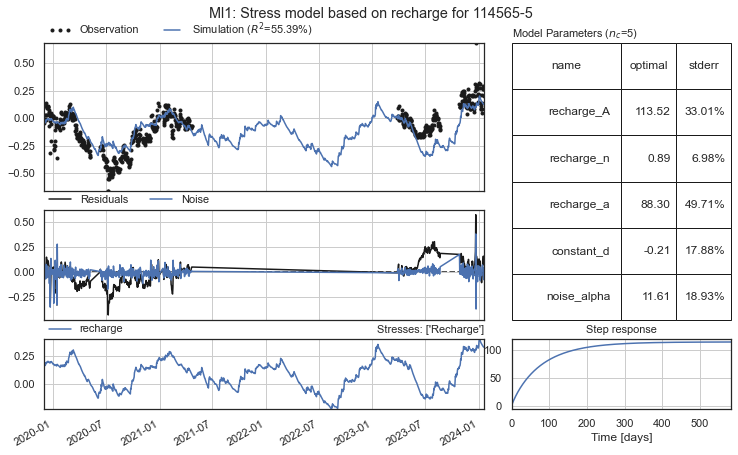
\includegraphics[width=\linewidth]{frontmatter/Rozenburg-fig/29.png}
        \caption{Monitoring well: 114565-5.}
        \label{fig:112565-3}
    \end{minipage}
    \hfill
\end{figure}\\

\newpage

\subsection{Stress Model 1: Heijplaat}\\
\\
\begin{figure}[htbp]
    \centering
    % First figure
    \begin{minipage}{0.32\textwidth}
        \centering
        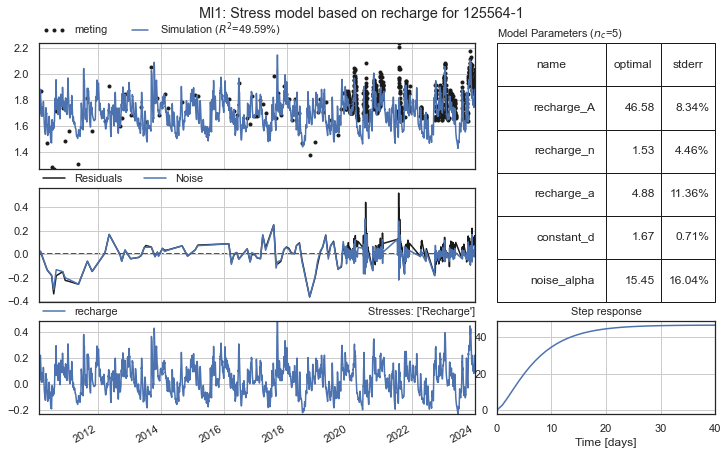
\includegraphics[width=\linewidth]{frontmatter/Heijplaat-fig/1.png}
        \caption{Monitoring well: 125564-1.}
        \label{SM: 125564-1}
    \end{minipage}
    \hfill
    % Second figure
    \begin{minipage}{0.32\textwidth}
        \centering
        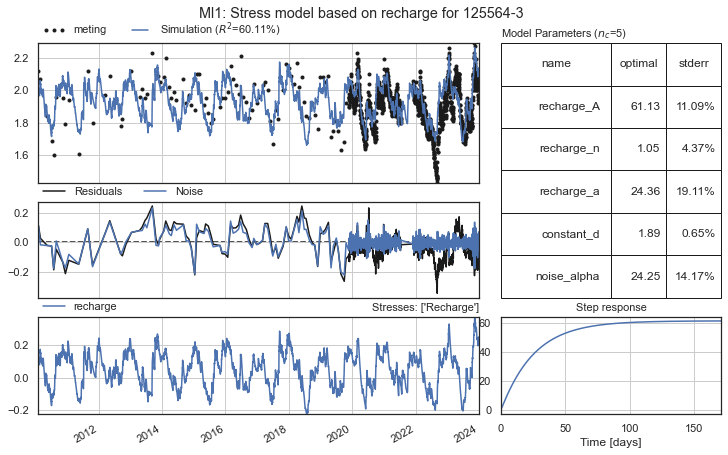
\includegraphics[width=\linewidth]{frontmatter/Heijplaat-fig/2.png}
        \caption{Monitoring well: 125564-3.}
        \label{SM: 125564-3}
    \end{minipage}
    \hfill
    % Third figure
    \begin{minipage}{0.32\textwidth}
        \centering
        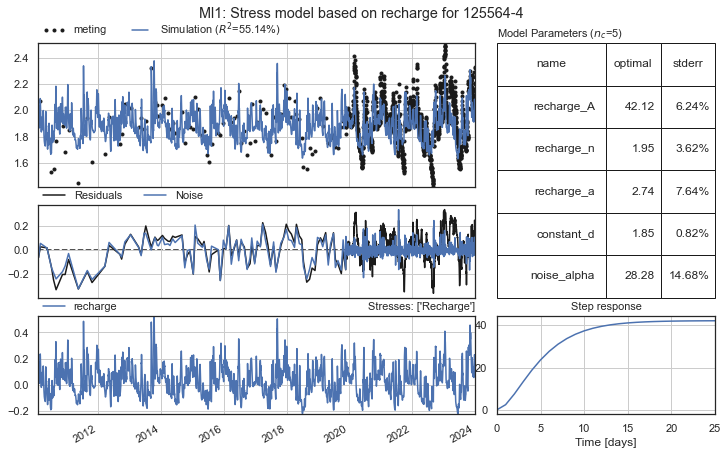
\includegraphics[width=\linewidth]{frontmatter/Heijplaat-fig/3.png}
        \caption{Monitoring well: 125564-4.}
        \label{SM: 125564-4}
    \end{minipage}
\end{figure}
\begin{figure}[htbp]
    \centering
    % First figure
    \begin{minipage}{0.32\textwidth}
        \centering
        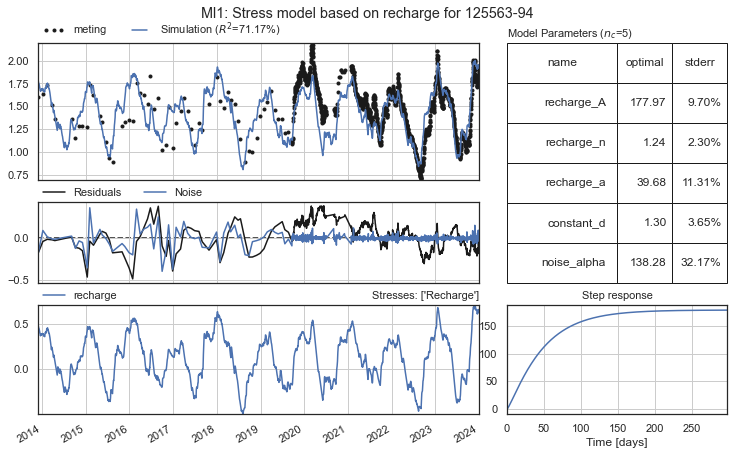
\includegraphics[width=\linewidth]{frontmatter/Heijplaat-fig/4.png}
        \caption{Monitoring well: 125563-94.}
        \label{SM:125563-94}
    \end{minipage}
    \hfill
    % Second figure
    \begin{minipage}{0.32\textwidth}
        \centering
        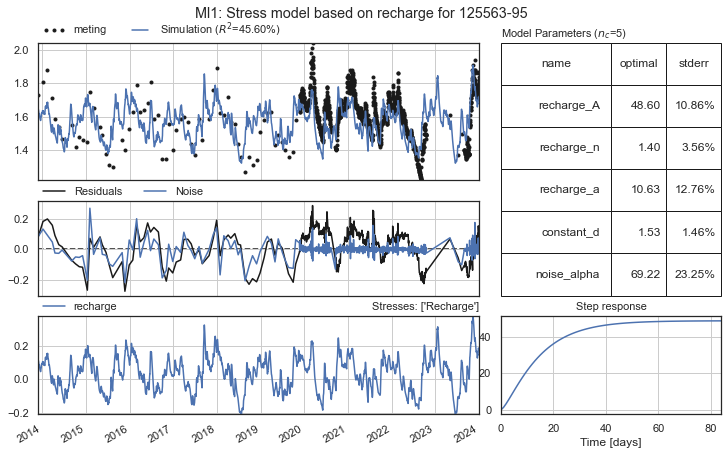
\includegraphics[width=\linewidth]{frontmatter/Heijplaat-fig/5.png}
        \caption{Monitoring well: 125563-95.}
        \label{SM: 125563-95}
    \end{minipage}
    \hfill
    % Third figure
    \begin{minipage}{0.32\textwidth}
        \centering
        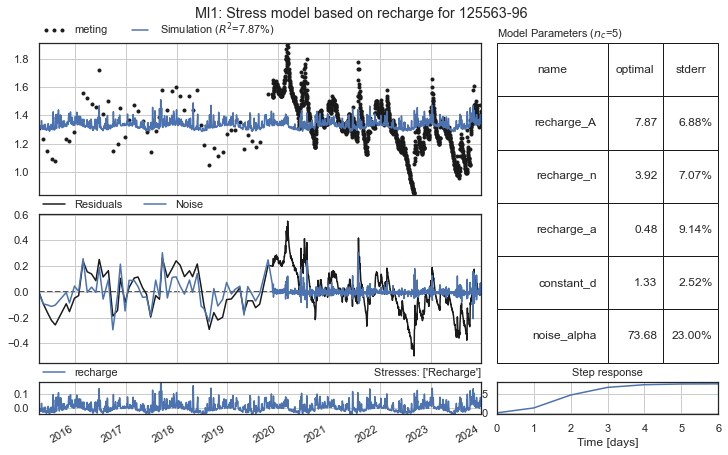
\includegraphics[width=\linewidth]{frontmatter/Heijplaat-fig/6.png}
        \caption{Monitoring well: 125563-96.}
        \label{SM: 125563-96}
    \end{minipage}
\end{figure}

\begin{figure}[htbp]
    \centering
    % First figure
    \begin{minipage}{0.32\textwidth}
        \centering
        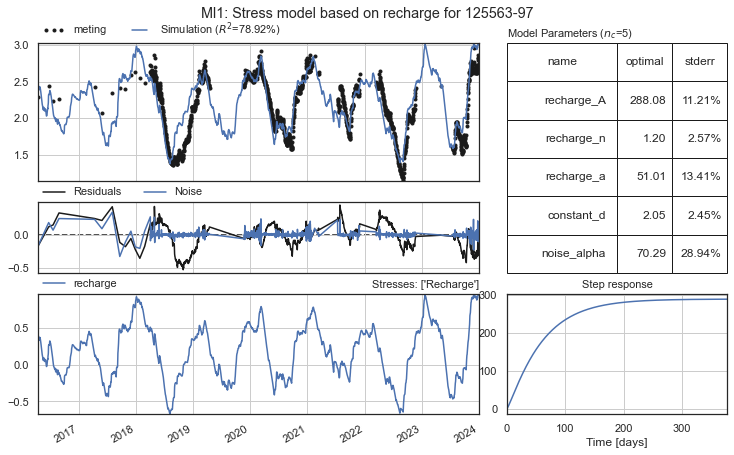
\includegraphics[width=\linewidth]{frontmatter/Heijplaat-fig/7.png}
        \caption{Monitoring well: 125563-97.}
        \label{SM: 125563-97}
    \end{minipage}
    \hfill
    % Second figure
    \begin{minipage}{0.32\textwidth}
        \centering
        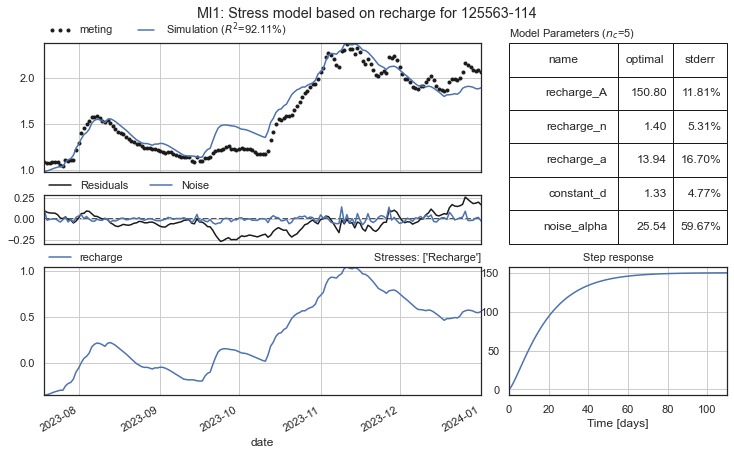
\includegraphics[width=\linewidth]{frontmatter/Heijplaat-fig/ml125563114.png}
        \caption{Verander: Monitoring well: 125564-114.}
        \label{SM: 125564-3}
    \end{minipage}
    \hfill
    % Third figure
    \begin{minipage}{0.32\textwidth}
        \centering
        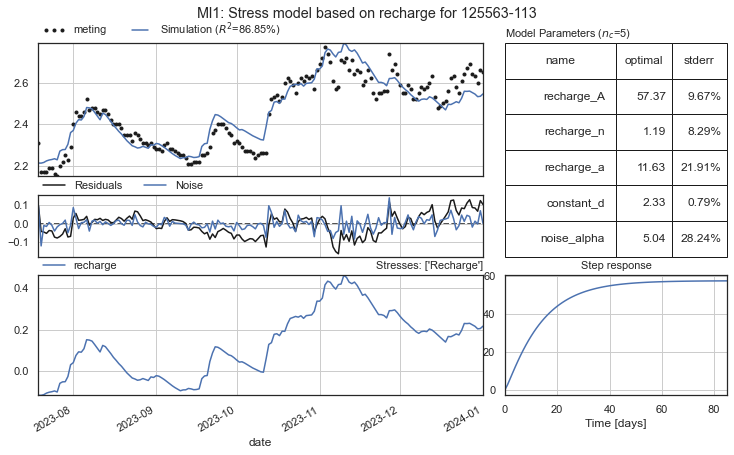
\includegraphics[width=\linewidth]{frontmatter/Heijplaat-fig/9.png}
        \caption{Monitoring well: 125563-113.}
        \label{SM: 125563-113}
    \end{minipage}
\end{figure}

\begin{figure}[htbp]
    \centering
    % First figure
    \begin{minipage}{0.32\textwidth}
        \centering
        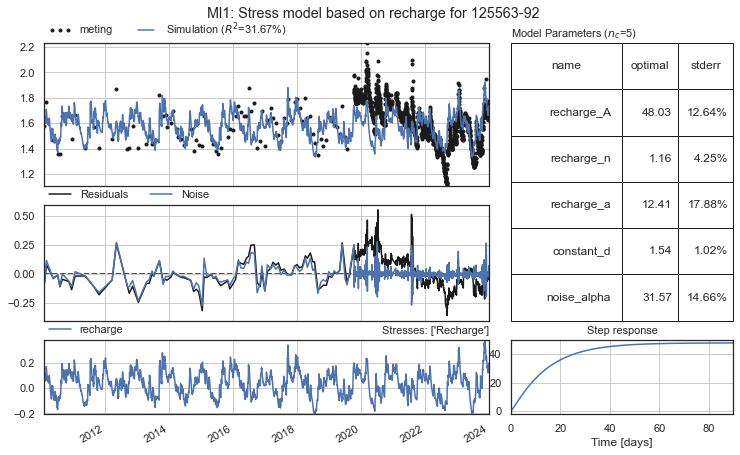
\includegraphics[width=\linewidth]{frontmatter/Heijplaat-fig/10.png}
        \caption{Monitoring well: 125563-92.}
        \label{SM: 125563-92}
    \end{minipage}
    \hfill
    % Second figure
    \begin{minipage}{0.32\textwidth}
        \centering
        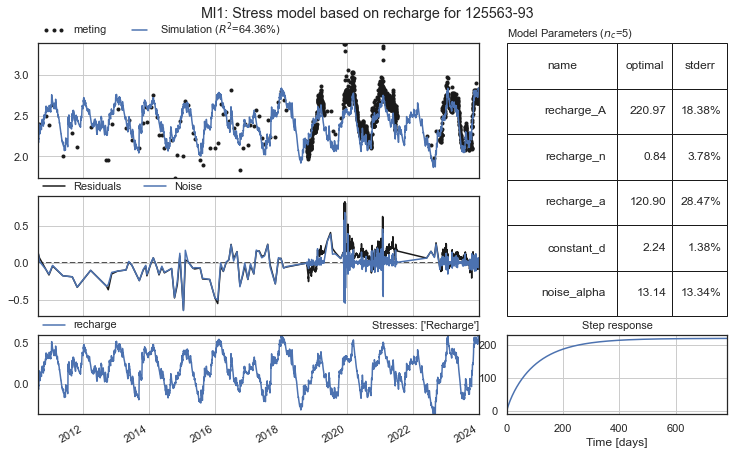
\includegraphics[width=\linewidth]{frontmatter/Heijplaat-fig/11.png}
        \caption{Monitoring well: 125563-93.}
        \label{SM: 125563-93}
    \end{minipage}
    \hfill
    % Third figure
    \begin{minipage}{0.32\textwidth}
        \centering
        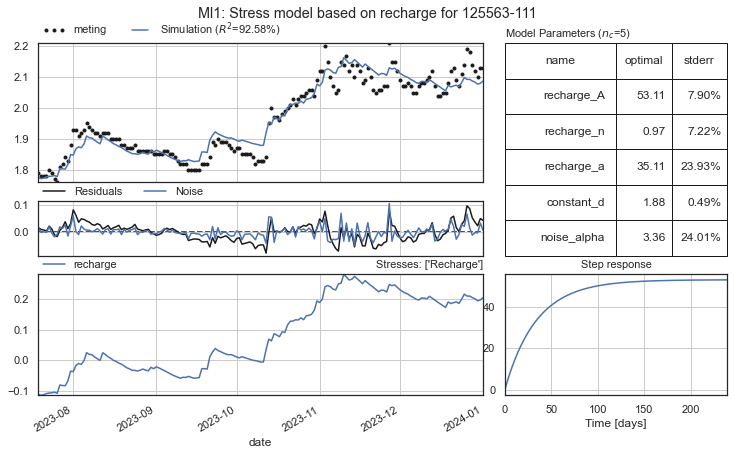
\includegraphics[width=\linewidth]{frontmatter/Heijplaat-fig/12.png}
        \caption{Monitoring well: 125563-111.}
        \label{SM: 125563-111}
    \end{minipage}
\end{figure}

\begin{figure}[htbp]
    \centering
    % First figure
    \begin{minipage}{0.32\textwidth}
        \centering
        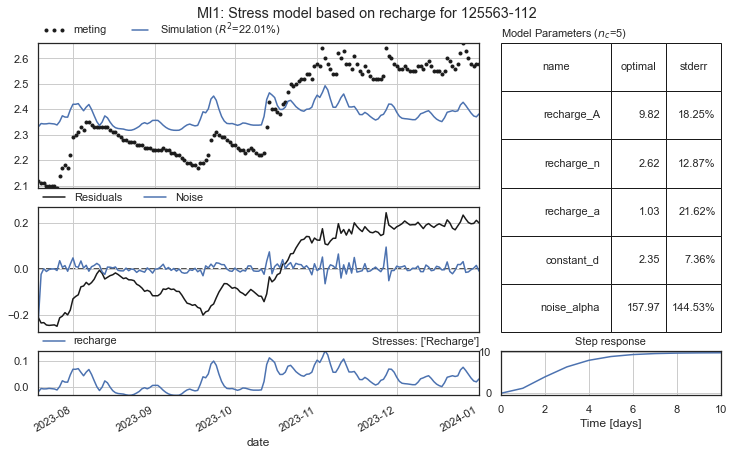
\includegraphics[width=\linewidth]{frontmatter/Heijplaat-fig/13.png}
        \caption{Monitoring well: 125563-112.}
        \label{SM: 125563-112}
    \end{minipage}
    \hfill
    % Second figure
    \begin{minipage}{0.32\textwidth}
        \centering
        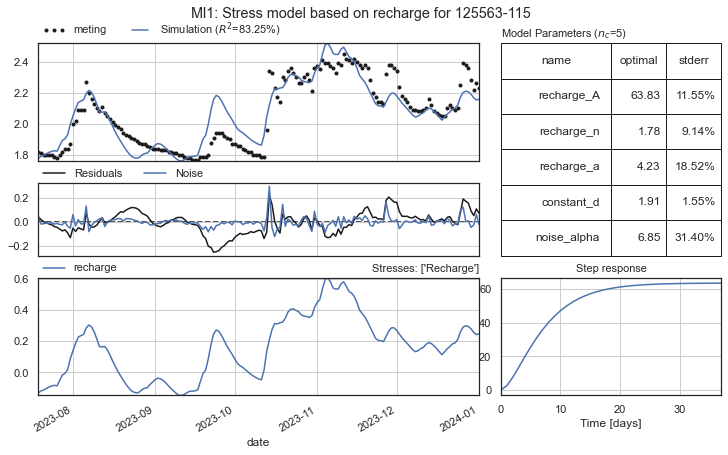
\includegraphics[width=\linewidth]{frontmatter/Heijplaat-fig/ml1125563115.png}
        \caption{Monitoring well: 125563-115.}
        \label{SM: 125563-115}
    \end{minipage}  
\end{figure}\\



































\newpage
\subsection{Stress Model 2: Rozenburg}\\
\\
\begin{figure}[htbp]
    \centering
    % First figure
    \begin{minipage}{0.32\textwidth}
        \centering
        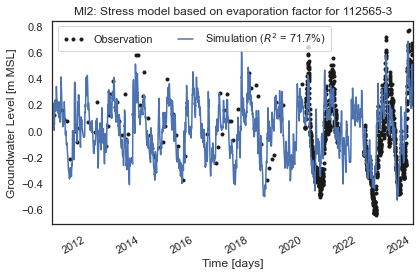
\includegraphics[width=\linewidth]{frontmatter/Rozenburg-fig/1125653.png}
        \caption{Monitoring well: 112565-3.}
        \label{SM2: start}
    \end{minipage}
    \hfill
    % Second figure
    \begin{minipage}{0.32\textwidth}
        \centering
        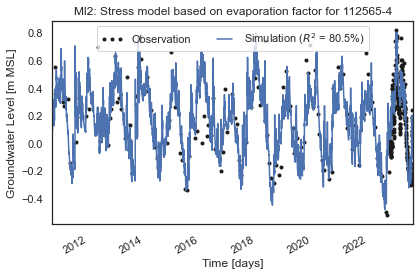
\includegraphics[width=\linewidth]{frontmatter/Rozenburg-fig/1125654.png}
        \caption{Monitoring well: 112565-4.}
        \label{fig:112565-4}
    \end{minipage}
    \hfill
    % Third figure
    \begin{minipage}{0.32\textwidth}
        \centering
        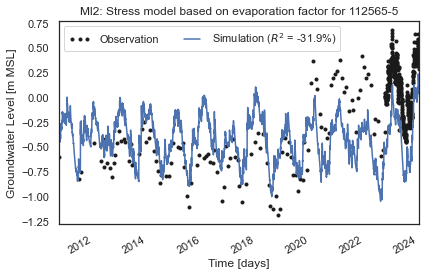
\includegraphics[width=\linewidth]{frontmatter/Rozenburg-fig/1125655.png}
        \caption{Monitoring well: 112565-5.}
        \label{fig:112565-5}
    \end{minipage}
\end{figure}

\begin{figure}[htbp]
    \centering
    % First figure
    \begin{minipage}{0.32\textwidth}
        \centering
        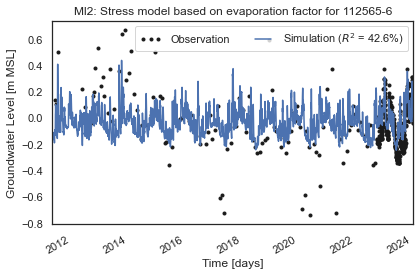
\includegraphics[width=\linewidth]{frontmatter/Rozenburg-fig/1125656(2).png}
        \caption{Monitoring well: 112565-6.}
        \label{fig:112565-6}
    \end{minipage}
    \hfill
    % Second figure
    \begin{minipage}{0.32\textwidth}
        \centering
        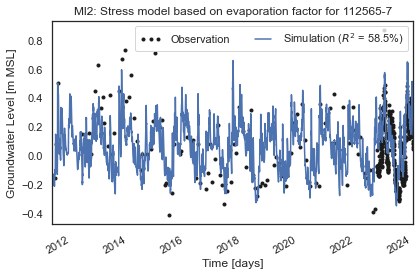
\includegraphics[width=\linewidth]{frontmatter/Rozenburg-fig/1125657(2).png}
        \caption{Monitoring well: 112565-7}
        \label{fig:112565-7}
    \end{minipage}
    \hfill
    % Third figure
    \begin{minipage}{0.32\textwidth}
        \centering
        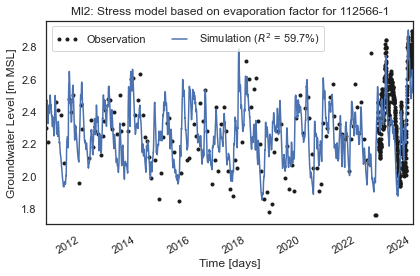
\includegraphics[width=\linewidth]{frontmatter/Rozenburg-fig/1125661.png}
        \caption{Monitoring well: 112566-1.}
        \label{fig:112566-1}
    \end{minipage}
\end{figure}

\begin{figure}[htbp]
    \centering
    % First figure
    \begin{minipage}{0.32\textwidth}
        \centering
        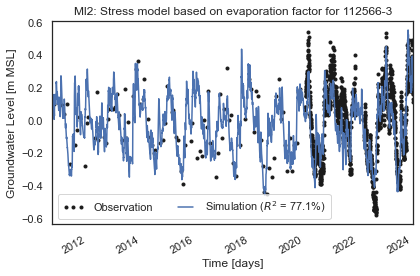
\includegraphics[width=\linewidth]{frontmatter/Rozenburg-fig/1125663.png}
        \caption{Monitoring well: 112566-3.}
        \label{fig:112566-3.}
    \end{minipage}
    \hfill
    % Second figure
    \begin{minipage}{0.32\textwidth}
        \centering
        \includegraphics[width=\linewidth]{frontmatter/Rozenburg-fig/1125665.png}
        \caption{Monitoring well: 112566-5.}
        \label{fig:112566-5}
    \end{minipage}
    \hfill
    % Third figure
    \begin{minipage}{0.32\textwidth}
        \centering
        \includegraphics[width=\linewidth]{frontmatter/Rozenburg-fig/1125656(2).png}
        \caption{Monitoring well: 112565-6.}
        \label{fig:112565-6}
    \end{minipage}
\end{figure}
\begin{figure}[htbp]
    \centering
    % First figure
    \begin{minipage}{0.32\textwidth}
        \centering
        \includegraphics[width=\linewidth]{frontmatter/Rozenburg-fig/1125657(2).png}
        \caption{Monitoring well: 112565-7.}
        \label{fig:112565-7}
    \end{minipage}
    \hfill
    % Second figure
    \begin{minipage}{0.32\textwidth}
        \centering
        \includegraphics[width=\linewidth]{frontmatter/Rozenburg-fig/1125661.png}
        \caption{Monitoring well: 112566-1.}
        \label{fig:112566-1}
    \end{minipage}
    \hfill
    % Third figure
    \begin{minipage}{0.32\textwidth}
        \centering
        \includegraphics[width=\linewidth]{frontmatter/Rozenburg-fig/1125663.png}
        \caption{Monitoring well: 112566-3.}
        \label{fig:112566-3}
    \end{minipage}
\end{figure}

\begin{figure}[htbp]
    \centering
    % First figure
    \begin{minipage}{0.32\textwidth}
        \centering
        \includegraphics[width=\linewidth]{frontmatter/Rozenburg-fig/1125665.png}
        \caption{Monitoring well: 112566-5.}
        \label{fig:112566-5}
    \end{minipage}
    \hfill
    % Second figure
    \begin{minipage}{0.32\textwidth}
        \centering
        \includegraphics[width=\linewidth]{frontmatter/Rozenburg-fig/1125666.png}
        \caption{Monitoring well: 112566-6.}
        \label{fig:112566-6}
    \end{minipage}
    \hfill
    % Third figure
    \begin{minipage}{0.32\textwidth}
        \centering
        \includegraphics[width=\linewidth]{frontmatter/Rozenburg-fig/1125668(2).png}
        \caption{Monitoring well: 112566-8.}
        \label{fig:112566-8}
    \end{minipage}
\end{figure}
\begin{figure}[htbp]
    \centering
    % First figure
    \begin{minipage}{0.32\textwidth}
        \centering
        \includegraphics[width=\linewidth]{frontmatter/Rozenburg-fig/1135643(2).png}
        \caption{Monitoring well: 113564-3.}
        \label{fig:113564-3}
    \end{minipage}
    \hfill
    % Second figure
    \begin{minipage}{0.32\textwidth}
        \centering
        \includegraphics[width=\linewidth]{frontmatter/Rozenburg-fig/1135651.png}
        \caption{Monitoring well: 113565-1.}
        \label{fig:113565-1}
    \end{minipage}
    \hfill
    % Third figure
    \begin{minipage}{0.32\textwidth}
        \centering
        \includegraphics[width=\linewidth]{frontmatter/Rozenburg-fig/1135652(2)png.png}
        \caption{Monitoring well: 113565-2.}
        \label{fig:113565-2}
    \end{minipage}
\end{figure}
\begin{figure}[htbp]
    \centering
    % First figure
    \begin{minipage}{0.32\textwidth}
        \centering
        \includegraphics[width=\linewidth]{frontmatter/Rozenburg-fig/1135653.png}
        \caption{Monitoring well: 113565-3.}
        \label{fig:113565-3}
    \end{minipage}
    \hfill
    % Second figure
    \begin{minipage}{0.32\textwidth}
        \centering
        \includegraphics[width=\linewidth]{frontmatter/Rozenburg-fig/1135654.png}
        \caption{Monitoring well: 113565-4.}
        \label{fig:113565-4}
    \end{minipage}
    \hfill
    % Third figure
    \begin{minipage}{0.32\textwidth}
        \centering
        \includegraphics[width=\linewidth]{frontmatter/Rozenburg-fig/1135655.png}
        \caption{Monitoring well: 113565-5.}
        \label{fig:113565-5}
    \end{minipage}
\end{figure}
\begin{figure}[htbp]
    \centering
    % First figure
    \begin{minipage}{0.32\textwidth}
        \centering
        \includegraphics[width=\linewidth]{frontmatter/Rozenburg-fig/1135656.png}
        \caption{Monitoring well: 113565-6.}
        \label{fig:113565-6}
    \end{minipage}
    \hfill
    % Second figure
    \begin{minipage}{0.32\textwidth}
        \centering
        \includegraphics[width=\linewidth]{frontmatter/Rozenburg-fig/1135657.png}
        \caption{Monitoring well: 113565-7.}
        \label{fig:113565-7}
    \end{minipage}
    \hfill
    % Third figure
    \begin{minipage}{0.32\textwidth}
        \centering
        \includegraphics[width=\linewidth]{frontmatter/Rozenburg-fig/1135658.png}
        \caption{Monitoring well: 113565-8.}
        \label{fig:113565-8}
    \end{minipage}
\end{figure}
\begin{figure}[htbp]
    \centering
    % First figure
    \begin{minipage}{0.32\textwidth}
        \centering
        \includegraphics[width=\linewidth]{frontmatter/Rozenburg-fig/1135661.png}
        \caption{Monitoring well: 113566-1.}
        \label{fig:113566-1}
    \end{minipage}
    \hfill
    % Second figure
    \begin{minipage}{0.32\textwidth}
        \centering
        \includegraphics[width=\linewidth]{frontmatter/Rozenburg-fig/1145642(2).png}
        \caption{Monitoring well: 114564-2.}
        \label{fig:114564-2}
    \end{minipage}
    \hfill
    % Third figure
    \begin{minipage}{0.32\textwidth}
        \centering
        \includegraphics[width=\linewidth]{frontmatter/Rozenburg-fig/1145643.png}
        \caption{Monitoring well: 114564-3.}
        \label{fig:114564-3}
    \end{minipage}
\end{figure}

\begin{figure}[htbp]
    \centering
    % First figure
    \begin{minipage}{0.32\textwidth}
        \centering
        \includegraphics[width=\linewidth]{frontmatter/Rozenburg-fig/1145647.png}
        \caption{Monitoring well: 114564-7.}
        \label{fig:114564-7}
    \end{minipage}
    \hfill
    % Second figure
    \begin{minipage}{0.32\textwidth}
        \centering
        \includegraphics[width=\linewidth]{frontmatter/Rozenburg-fig/1145651(2).png}
        \caption{Monitoring well: 114565-1.}
        \label{fig:114565-1}
    \end{minipage}
    \hfill
\end{figure}\\
\newpage
\\
\subsection{Stress Model 2: Heijplaat}\\
\\
\begin{figure}[htbp]
    \centering
    % First figure
    \begin{minipage}{0.32\textwidth}
        \centering
        \includegraphics[width=\linewidth]{frontmatter/Heijplaat-fig/12556-111.png}
        \caption{Monitoring well: 125563-111.}
        \label{SM: 125563-111}
    \end{minipage}
    \hfill
    % Second figure
    \begin{minipage}{0.32\textwidth}
        \centering
        \includegraphics[width=\linewidth]{frontmatter/Heijplaat-fig/125563-92.png}
        \caption{Monitoring well: 125563-92.}
        \label{SM: 125563-92}
    \end{minipage}
    \hfill
    % Third figure
    \begin{minipage}{0.32\textwidth}
        \centering
        \includegraphics[width=\linewidth]{frontmatter/Heijplaat-fig/125563-93.png}
        \caption{Monitoring well: 125563-93.}
        \label{SM: 125563-93}
    \end{minipage}
\end{figure}
\begin{figure}[htbp]
    \centering
    % First figure
    \begin{minipage}{0.32\textwidth}
        \centering
        \includegraphics[width=\linewidth]{frontmatter/Heijplaat-fig/125563-94.png}
        \caption{Monitoring well: 125563-94.}
        \label{SM:125563-94}
    \end{minipage}
    \hfill
    % Second figure
    \begin{minipage}{0.32\textwidth}
        \centering
        \includegraphics[width=\linewidth]{frontmatter/Heijplaat-fig/125563-95.png}
        \caption{Monitoring well: 125563-95.}
        \label{SM: 125563-95}
    \end{minipage}
    \hfill
    % Third figure
    \begin{minipage}{0.32\textwidth}
        \centering
        \includegraphics[width=\linewidth]{frontmatter/Heijplaat-fig/125563-97.png}
        \caption{Monitoring well: 125563-97.}
        \label{SM: 125563-97}
    \end{minipage}
\end{figure}

\begin{figure}[htbp]
    \centering
    % First figure
    \begin{minipage}{0.32\textwidth}
        \centering
        \includegraphics[width=\linewidth]{frontmatter/Heijplaat-fig/125563-112.png}
        \caption{Monitoring well: 125563-112.}
        \label{SM: 125563-112}
    \end{minipage}
    \hfill
    % Second figure
    \begin{minipage}{0.32\textwidth}
        \centering
        \includegraphics[width=\linewidth]{frontmatter/Heijplaat-fig/125563-113.png}
        \caption{Monitoring well: 125563-113.}
        \label{SM: 125563-113}
    \end{minipage}
    \hfill
    % Third figure
    \begin{minipage}{0.32\textwidth}
        \centering
        \includegraphics[width=\linewidth]{frontmatter/Heijplaat-fig/12556396.png}
        \caption{Monitoring well: 125563-96.}
        \label{SM: 125563-113}
    \end{minipage}
\end{figure}

\begin{figure}[htbp]
    \centering
    % First figure
    \begin{minipage}{0.32\textwidth}
        \centering
        \includegraphics[width=\linewidth]{frontmatter/Heijplaat-fig/125563-114.png}
        \caption{Monitoring well: 125563-114.}
        \label{SM: 125563-114}
    \end{minipage}
    \hfill
    % Second figure
    \begin{minipage}{0.32\textwidth}
        \centering
        \includegraphics[width=\linewidth]{frontmatter/Heijplaat-fig/125563-115.png}
        \caption{Monitoring well: 125563-115.}
        \label{SM: 125563-115}
    \end{minipage}
    \hfill
    % Third figure
    \begin{minipage}{0.32\textwidth}
        \centering
        \includegraphics[width=\linewidth]{frontmatter/Heijplaat-fig/125564-3.png}
        \caption{Monitoring well: 125564-3.}
        \label{SM: 125564-3}
    \end{minipage}
\end{figure}

\begin{figure}[htbp]
    \centering
    % First figure
    \begin{minipage}{0.32\textwidth}
        \centering
        \includegraphics[width=\linewidth]{frontmatter/Heijplaat-fig/125564-4.png}
        \caption{Monitoring well: 125564-4.}
        \label{SM: 125563-114}
    \end{minipage}
    \hfill
    % Second figure
    \begin{minipage}{0.32\textwidth}
        \centering
        \includegraphics[width=\linewidth]{frontmatter/Heijplaat-fig/1255641.png}
        \caption{Monitoring well: 125564-1.}
        \label{SM: 125563-115}
    \end{minipage}
\end{figure}